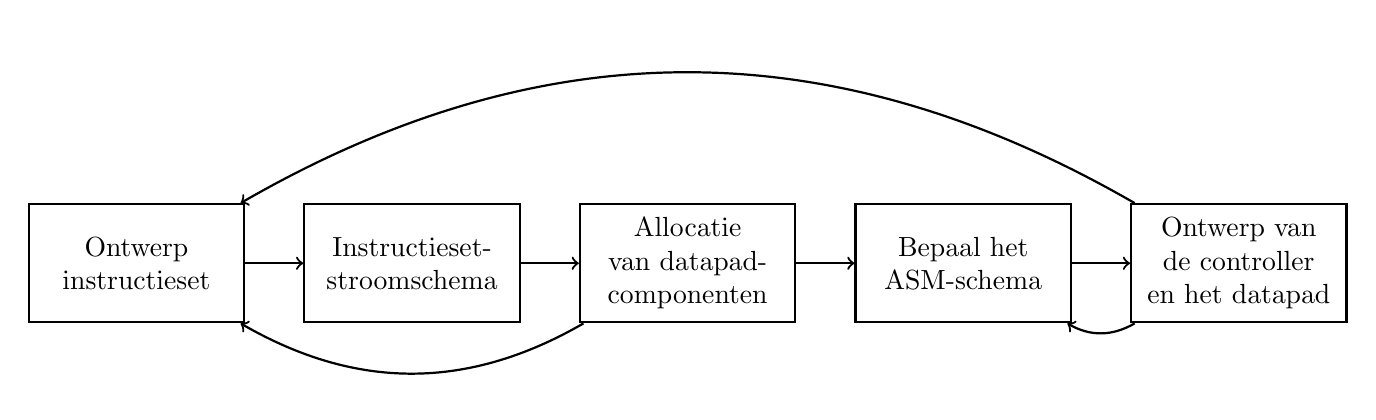
\begin{tikzpicture}[stage/.style={draw,rectangle,minimum width=2.5 cm, minimum height=1.5 cm,text width=2.5 cm,align=center,thick},tostage/.style={thick,->}]
\node[stage] (A) at (0,0) {Ontwerp instructieset};
\node[stage] (B) at (3.5,0) {Instructieset-stroomschema};
\node[stage] (C) at (7,0) {Allocatie van datapad\-componenten}
  edge  [bend left,tostage] (A);
\node[stage] (D) at (10.5,0) {Bepaal het ASM-schema};
\node[stage] (E) at (14,0) {Ontwerp van de controller en het datapad}
  edge  [bend left,tostage] (D)
  edge  [bend right,tostage] (A);
\draw[tostage] (A) -- (B);
\draw[tostage] (B) -- (C);
\draw[tostage] (C) -- (D);
\draw[tostage] (D) -- (E);
\end{tikzpicture}